% Chapter 2 Support Vector Machine

\chapter{پشینیه پژوهش}
\section{ماشین بردار پشتیبان}
در این بخش، ابتدا ماشین بردار پشتیبان خطی و غیر خطی شرح داده می‌شود. سپس پیشینه پژوهش در زمینه ماشین بردار پشتیبان بررسی می‌گردد.
\subsection{ماشین بردار پشتیبان با حاشیه سخت}
ماشین بردار پشتیبان با هدف جداسازی نمونه‌های دو کلاس در سال 1995 معرفی گردید \cite{vapnik1995}. ایده اصلی این روش یادگیری، بدست آوردن ابرصفحه بهینه‌ای است که از نمونه‌های دو کلاس تا جای ممکن بیشترین فاصله را داشته باشد. به عبارت دیگر، این روش یادگیری حاشیه دو کلاس را بیشینه می‌کند. برای فهم بهتر ایده این روش، فرض کنید مجموعه داده‌ی $T=\{(x_1, y_1),(x_2, y_2) \cdots , (x_m, y_m)\}$ را در اختیار داریم که شامل $m$ تا نمونه آموزشی است. هر نمونه آموزشی $x_{i} \in \mathbb{R}^{n}$ با $n$ ویژگی در فضای ورودی و $y_i \in \{-1,1\}$ برچسب نمونه‌ی $x_i$ می‌باشد. در ساده‌ترین حالت، نمونه‌های دو کلاس در مجموعه داده $T$ با یک ابرصفحه $w^{T}x+b$ بدون خطا دسته‌بندی می‌شود. این حالت مسئله حاشیه سخت\footnote{\lr{Hard margin}}  نامیده می‌شود. شکل \ref{fig:SVM-HM} مسئله حاشیه سخت در روش \lr{SVM} را نشان می‌دهد. (لازم به ذکر است، خطوط نقطه‌چین در شکل ‏\ref{fig:SVM-HM} نشان دهنده حاشیه است.) در این حالت، یک مسئله بهینه‌سازی برای بدست آوردن ابرصفحه باید حل گردد.

\begin{figure}[!t]
	\centering
	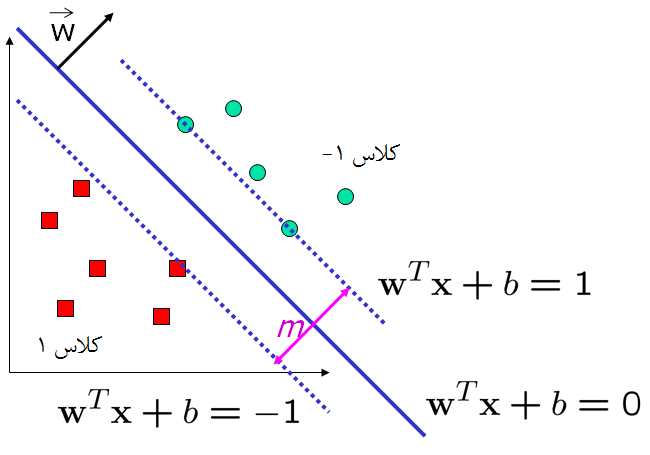
\includegraphics[scale=0.5]{SVM-HardMargin}
	\caption{مسئله حاشیه سخت در ماشین بردار پشتیبان}
	\label{fig:SVM-HM}
\end{figure}